\documentclass[11pt]{article}
\usepackage{acl}

\usepackage[T1]{fontenc}
\usepackage[utf8]{inputenc}
\usepackage{times}
\usepackage{latexsym}
\usepackage{microtype}
\usepackage{amsmath,amssymb}
\usepackage{graphicx}
\usepackage{booktabs}
\usepackage{multirow}
\usepackage{float}
\usepackage{url}
\usepackage{xurl}
\usepackage{tikz}
\hyphenation{Hy-brid-Ver-dict-Head}

\graphicspath{{figures/}}
% Auto-generated by analysis/aggregate.py — do not edit by hand
\newcommand{\BaselineMF}{0.385}
\newcommand{\BaselineStd}{0.007}
\newcommand{\VtwoMF}{0.918}
\newcommand{\VtwoStd}{0.017}
\newcommand{\VthreeMF}{0.907}
\newcommand{\VthreeStd}{0.019}
\newcommand{\GapMF}{0.533}
\newcommand{\LogBlindMF}{0.389}
\newcommand{\LogAwareMF}{0.882}
\newcommand{\LogAwareStd}{0.997}
\newcommand{\MidTierMF}{0.204}
\newcommand{\MidTierBlindMF}{0.016}
\newcommand{\AlwaysNEEMF}{0.250}
\newcommand{\ECHigh}{0.781}
\newcommand{\ECLowMax}{0.380}
\newcommand{\ECMidA}{0.426}
\newcommand{\ECMidB}{0.539}
\newcommand{\ECMidC}{0.639}
\newcommand{\VtwoMidMF}{0.252}
\newcommand{\VtwoMidStd}{0.024}
\newcommand{\VthreeMidMF}{0.237}
\newcommand{\VthreeMidStd}{0.026}
\newcommand{\VtwoStdMF}{1.000}
\newcommand{\VtwoVHAcc}{0.870}
\newcommand{\VthreeVHAcc}{0.852}
\newcommand{\VtwoVHErr}{47}
\newcommand{\VthreeVHErr}{53}
\newcommand{\VHTotal}{360}
\newcommand{\NTotal}{2200}
\newcommand{\NTrain}{1600}
\newcommand{\NTest}{600}
\newcommand{\NStandard}{480}
\newcommand{\NMidTier}{120}


\title{When Trust Doesn't Transfer: Diagnosing Source-Credibility Shortcuts in Fact Verification Models}

\author{Dheeraj Karki \\
  Independent Researcher \\
  \texttt{dheerajkarki1790@gmail.com} \And
  Aiswarya Konavoor \\
  Togo AI Labs \\
  \texttt{aiswarya@togolabs.ai}}

\begin{document}
\maketitle

\begin{abstract}
Fact-verification models weighted by source trustworthiness need evaluations that only a trust-using model can pass. We audit a representative source-trust system and find three failures: a synthetic split leaks the verdict through textual register (trust-blind accuracy 0.996), AVeriTeC accuracy equals the majority-class prior (macro-F1 0.265), and a simulation split is closed-world trivial. We construct a synthetic, controlled trust-isolating benchmark holding evidence text byte-identical across trust tiers with source category fixed. The result is a sharp inversion: the trust-blind baseline collapses to chance (macro-F1 \BaselineMF\,$\pm$\,\BaselineStd), while a trust-aware graph network wins (v2-HGNN \VtwoMF\,$\pm$\,\VtwoStd) and a logistic-regression probe with the trust scalar reaches \LogAwareMF. An NLI-enhanced variant (v3-NLI, \VthreeMF\,$\pm$\,\VthreeStd) scores below v2-HGNN because this benchmark fixes inference strength at 1.0, removing the axis NLI would otherwise improve. Mid-tier boundary probes ($\mathrm{ST}\in\{0.50,0.62,0.72\}$) further reveal that even a trust-aware probe collapses to macro-F1 \MidTierMF, confirming that scalar access alone is insufficient and trust must be reasoned over continuously. We release the benchmark and generator with this submission.
\end{abstract}

\section{Introduction}
Automated fact verification predicts whether a claim is supported, refuted, or unverifiable given retrieved evidence. A persistent failure mode is shortcut learning: models reach high accuracy by exploiting surface regularities rather than reasoning over evidence. The best known case is claim-only bias in FEVER, where a classifier that never reads the evidence nearly matches an evidence-aware model \citep{schuster2019debias}. A natural and well-motivated direction is to make verification \emph{source-aware}: identical text from a peer-reviewed article and from an anonymous post should not be treated identically, so evidence should be weighted by the trustworthiness of its source \citep{popat2018declare,baly2018factuality}.

This paper is about how that idea is \emph{measured}. To claim that a model uses source trust, one needs an evaluation that only a trust-using model can solve. The intuitive construction pairs the same claim with a high-trust and a low-trust source and labels the low-trust version not-enough-evidence. We show that a careful instance of this construction silently leaks the verdict, that the leakage makes a trust-blind model appear to succeed, and that a second common reporting choice, accuracy on a class-imbalanced benchmark, hides a majority-class predictor. We then show how to build an evaluation that does isolate source trust, and what changes when it is used.

Our study object is a representative source-trust FV system that computes a per-evidence epistemic confidence from source trust, an evidence-type weight, and an inference strength, and aggregates these into a verdict through a heterogeneous graph neural network with a symbolic and a neural decision layer. We audit its evaluation, find it does not measure what it claims, and rebuild the measurement. Figure~\ref{fig:construction} summarizes the corrected benchmark.

\textbf{Contributions.}
\begin{enumerate}
\item \textbf{A leakage diagnosis.} We show that a synthetic ``shortcut-breaking'' trust split leaks the verdict through textual register (a template field predicts it at 0.99 and a trust-blind model scores 0.996), that reporting AVeriTeC accuracy of 0.665 masks the majority-class prior (macro-F1 0.265), and that the simulation split is closed-world trivial (Section~\ref{sec:diagnosis}).
\item \textbf{A trust-isolating benchmark.} We construct a split that admits no detectable non-trust path to the label, and report the lesson that text isolation alone is insufficient: a first version still leaked at macro-F1 0.82 through the source-category proxy until the category was neutralized (Section~\ref{sec:benchmark}). The benchmark is deliberately single-evidence, single evidence-type (testimony), and single source-category; these constraints hold every axis except source trust constant so that results are attributable to trust alone.
\item \textbf{The inversion.} On the corrected benchmark a trust-blind model is at chance and a trust-aware model wins, the opposite of the leaky split, confirmed with both a controlled probe and the original graph network (Section~\ref{sec:experiments}).
\end{enumerate}
We release the benchmark generator and data so the construction can be inspected and extended.

\section{Background and Related Work}
\textbf{Fact-verification benchmarks.} FEVER introduced large-scale claim verification over Wikipedia with three verdict classes \citep{thorne2018fever}. AVeriTeC moved to real-world claims with web evidence and four verdict classes, and is heavily skewed toward the refuted class \citep{schlichtkrull2023averitec}. AVeriTeC distinguishes plain verdict accuracy from an evidence-gated score; we use it only as a verdict-accuracy testbed and report macro-F1 against the majority baseline, because the class skew makes accuracy alone uninformative.

\textbf{Shortcuts and robustness in FV.} Claim-only bias was documented for FEVER together with a symmetric evaluation set \citep{schuster2019debias}. Annotation artifacts --- surface patterns in hypotheses that predict labels without evidence --- are a broader class of the same problem \citep{gururangan2018annotation}, and hypothesis-only baselines have exposed such artifacts in NLI benchmarks \citep{poliak2018hypothesis}. VitaminC built contrastive evidence pairs that force a model to read the evidence rather than the claim \citep{schuster2021vitaminc}. These works target lexical and evidence-content shortcuts. The shortcut we study is different: a model can recover the verdict from the \emph{register} of the evidence text, which is correlated with source trust by construction. Our corrected benchmark instantiates the contrast-set principle \citep{gardner2020evaluating} --- a paired set of records differing in exactly one signal, so that a model can pass only by reading that signal --- specialised to the source-trust axis.

\textbf{Source-credibility verification.} DeClarE weighted evidence with a learned source-trustworthiness representation for claim credibility \citep{popat2018declare}. Source factuality has been predicted at the outlet level from multiple signals \citep{baly2018factuality}. These supply or use a trust signal but do not provide a measurement that isolates it; our contribution is the isolating evaluation.

\textbf{Graph and symbolic FV.} Evidence aggregation over graphs is a standard FV backbone, from GEAR \citep{zhou2019gear} and the kernel graph attention network \citep{liu2020kgat} to stance-aware aggregation \citep{si2021tarsa} and heterogeneous-graph reasoning over text and tables \citep{gong2024heterfc}. Knowledge-graph-based grounding checks have been applied to detect hallucinations in LLM outputs \citep{sansford2024grapheval}, and logic-regularized models give interpretable, auditable verdicts \citep{chen2022loren}. The system we audit sits in this family; our focus is its evaluation, not its architecture. Epistemology-grounded reasoning in language models is nascent and, to date, targets general deduction rather than fact verification \citep{sathish2026pramana}.

\section{The System Under Study}
\label{sec:system}
The audited system is a prior implementation \citep{karki2026system}; its leaky-split, AVeriTeC, and simulation numbers (the Original split row of Table~\ref{tab:inversion} and the upper rows of Table~\ref{tab:diagnosis}) are taken from that implementation's evaluation logs, with the corrected benchmark released with this submission. We treat the system as the study object rather than patching it in place: the benchmark contribution is separable from, and portable beyond, the specific architecture that prompted it. The system assigns each evidence item an epistemic confidence
\begin{equation}
\mathrm{EC}_i = 1 - (1 - \mathrm{ST}_i)^{\,\mathrm{EW}_i \cdot \mathrm{IS}_i},
\label{eq:ec}
\end{equation}
where $\mathrm{ST}_i \in [0,1]$ is a registry-assigned source-trust score, $\mathrm{EW}_i \in [0,1]$ is an evidence-type weight (testimony: 0.80; perception: 0.95; inference by analogy: 0.55), and $\mathrm{IS}_i \in [0,1]$ is an inference strength. The single-evidence verdict rule is: if $\mathrm{EC}_i \geq 0.75$ and the evidence supports the claim, output \textsc{supported}; if $\mathrm{EC}_i \geq 0.75$ and the evidence refutes it, output \textsc{refuted}; otherwise output \textsc{not\_enough\_evidence} (this rule defines the benchmark data labels; the trained model's inference path is described in Section~\ref{sec:experiments}). This threshold grounds the three tiers of the corrected benchmark: high-trust sources ($\mathrm{ST}\geq 0.85$, $\mathrm{EW}=0.80$, $\mathrm{IS}=1.0$) yield $\mathrm{EC}\geq \ECHigh>0.75$ and receive a definitive verdict; low-trust sources ($\mathrm{ST}\leq 0.45$) yield $\mathrm{EC}\leq \ECLowMax<0.75$ and receive \textsc{nee}; mid-tier sources ($\mathrm{ST}\in\{0.50,0.62,0.72\}$) yield $\mathrm{EC}\in\{\ECMidA,\ECMidB,\ECMidC\}$, all below 0.75, and are used as boundary probes to test whether a model reasons continuously rather than learning a binary threshold.

Per-claim evidence is encoded by a heterogeneous graph network \citep{schlichtkrull2018rgcn} (graph attention \citep{velickovic2018gat} over claim and evidence nodes) with stance and inference-strength heads, and the verdict is produced either by a symbolic threshold on the aggregated $\mathrm{EC}$ or by a learned verdict head. For this study the relevant property of Eq.~\eqref{eq:ec} is monotonicity in $\mathrm{ST}$: with evidence type and inference strength fixed, raising source trust raises confidence. A model that ignores $\mathrm{ST}$ has no access to this signal. Figure~\ref{fig:ec_curve} visualises the formula.

\begin{figure}[t]
\centering

\includegraphics[width=\columnwidth]{figures/pb_ec_curve.png}
\caption{EC as a function of source trust $S_T$ for the three evidence-type weights. The red dotted line marks the decision threshold (EC~=~0.75). Coloured dots show the benchmark tier values. High-trust sources ($S_T\geq 0.85$, testimony curve) clear the threshold; low-trust ($S_T\leq 0.45$) fall well below it; mid-tier probes ($S_T\in\{0.50,0.62,0.72\}$) sit in the gap between the two zones, all still below 0.75.}
\label{fig:ec_curve}
\end{figure}

\section{Diagnosis: The Original Evaluation Does Not Measure Source Trust}
\label{sec:diagnosis}
We evaluate three claims in the original setup and find each undermined by its own data. Table~\ref{tab:diagnosis} collects the numbers.

\textbf{The synthetic split leaks through text register.} The synthetic ``shortcut-breaking'' split pairs claims with high- and low-trust sources and labels low-trust supporting text as not-enough-evidence, so that, in principle, only source trust can separate the pair. In practice the generator draws low-trust evidence from a rumour register (for example, ``An anonymous post claimed that\dots'') and high-trust evidence from an official register (``published findings confirming\dots''). Because the register is determined by the trust tier and the trust tier determines the verdict, the text register determines the verdict. A single-feature lookup confirms this: a per-record template field predicts the verdict at 0.99 (the field value encodes verdict, trust tier, and source identity simultaneously --- e.g., \texttt{high\_trust\_supported},\allowbreak\ \texttt{low\_trust\_nee} --- so 13 of 14 template types are 100\% predictive), the source identifier at 0.82, and the raw evidence text and its stance at 0.92 and 0.54 respectively (Table~\ref{tab:diagnosis}, Figure~\ref{fig:leakage}). Consequently, a trust-blind model that reads only the text reaches 0.996 accuracy on this split, and the trust-aware model scores lower (0.889), because the leaky split rewards reading the register rather than reasoning about the source.

\textbf{AVeriTeC accuracy hides the class prior.} The AVeriTeC subset is heavily imbalanced. The system maps AVeriTeC's four verdict classes to three (supported, refuted, not-enough-evidence). On this development set, always predicting the majority class (refuted) yields accuracy 0.660 and macro-F1 0.265. A standard text classifier collapses onto the majority class, predicting the not-enough-evidence class exactly once out of 462 examples, for accuracy 0.656 and macro-F1 0.354. The reported system accuracy of 0.665 lies on this prior; without macro-F1 it cannot be distinguished from a majority predictor.

\textbf{The simulation split is closed-world trivial.} The simulation split is drawn from AI2-THOR \citep{kolve2017ai2thor}, an interactive 3-D environment that provides closed-world ground truth for object and state claims. On this split, every evidence item has the same maximal source trust and evidence-type weight, so Eq.~\eqref{eq:ec} carries no discriminative signal, and the verdict is recoverable by matching a numeric value against simulator ground truth. Accuracy is 1.000, which reflects task triviality rather than epistemic reasoning, and inflates any average that includes it.

\begin{table}[t]
\caption{Diagnosis of the original evaluation. Each row reports a number that undercuts a source-trust claim. Lookup values are the fraction of verdicts recovered from a single non-trust feature.}
\label{tab:diagnosis}
\centering
\resizebox{\columnwidth}{!}{%
\begin{tabular}{@{}llr@{}}
\toprule
Finding & Measure & Value \\
\midrule
Synthetic: template field & verdict lookup & 0.99 \\
Synthetic: source id & verdict lookup & 0.82 \\
Synthetic: trust-blind model & accuracy $\uparrow$ & 0.996 \\
AVeriTeC: majority baseline & accuracy / macro-F1 & 0.660 / 0.265 \\
AVeriTeC: text classifier & accuracy / macro-F1 & 0.656 / 0.354 \\
Simulation split & accuracy $\uparrow$ & 1.000 \\
\bottomrule
\end{tabular}%
}
\end{table}

\section{A Trust-Isolating Benchmark}
\label{sec:benchmark}
We rebuild the evaluation so that source trust is the only feature that determines the label. Figure~\ref{fig:construction} shows the construction.

\textbf{Trust-isolation criterion.} A benchmark is \emph{trust-isolating} if (i) every non-trust input feature takes the same value for both records in each source-trust pair, and (ii) no single non-trust feature predicts the verdict above chance on the test set. The corrected benchmark satisfies both conditions (Table~\ref{tab:isolation}); we verify this empirically after construction.

\textbf{Design.} For each claim we generate one neutral evidence sentence and attach it, byte-identical, to a high-trust and a low-trust source. The verdict is derived from the system's own confidence rule, Eq.~\eqref{eq:ec}: with a single testimony item, high trust ($\mathrm{ST}\geq 0.85$) yields supported or refuted, and low trust ($\mathrm{ST}\leq 0.45$) yields not-enough-evidence. The text is therefore constant within each high/low pair, and only the source-trust scalar flips the label. The benchmark has \NTotal\ records, \NTrain\ for training and \NTest\ held out for test (\NStandard\ standard pairs plus \NMidTier\ mid-tier boundary probes); Figure~\ref{fig:tiers} shows the three ST zones. Table~\ref{tab:example} shows a concrete paired record.

\begin{table}[h]
\caption{Paired record from the benchmark. \textit{Claim}: ``The Velora battery cell output is 318 megawatts.'' \textit{Evidence}: ``Recorded measurements state that the Velora battery cell output is 318 megawatts.'' Evidence text is byte-identical in both rows; only ST changes, flipping the verdict.}
\label{tab:example}
\centering
\small
\begin{tabular}{@{}lccc@{}}
\toprule
Source & ST & EC & Verdict \\
\midrule
nm\_h85a (high-trust) & 0.85 & \ECHigh & {\normalfont\textsc{supported}} \\
nm\_l30a (low-trust)  & 0.30 & 0.248 & {\normalfont\textsc{nee}} \\
\bottomrule
\end{tabular}
\end{table}

\begin{figure}[!ht]
\centering
\resizebox{\columnwidth}{!}{%
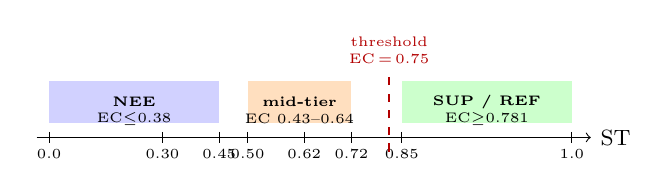
\begin{tikzpicture}[font=\footnotesize, xscale=0.80]
  \draw[->] (-0.2,0) -- (8.6,0) node[right] {$\mathrm{ST}$};
  \foreach \x/\lab in {0/0.0, 1.8/0.30, 2.7/0.45, 3.15/0.50, 4.05/0.62, 4.8/0.72, 5.6/0.85, 8.3/1.0} {
    \draw (\x,0.07) -- (\x,-0.07);
    \node[below=1pt, font=\tiny] at (\x,0) {\lab};
  }
  \fill[blue!18] (0,0.18) rectangle (2.7,0.72);
  \node[font=\tiny\bfseries] at (1.35,0.45) {NEE};
  \node[font=\tiny] at (1.35,0.24) {EC$\leq$0.38};
  \fill[orange!25] (3.15,0.18) rectangle (4.8,0.72);
  \node[font=\tiny\bfseries] at (3.975,0.45) {mid-tier};
  \node[font=\tiny] at (3.975,0.24) {EC 0.43--0.64};
  \fill[green!20] (5.6,0.18) rectangle (8.3,0.72);
  \node[font=\tiny\bfseries] at (6.95,0.45) {SUP / REF};
  \node[font=\tiny] at (6.95,0.24) {EC$\geq$0.781};
  \draw[dashed, red!70!black, thick] (5.4,-0.18) -- (5.4,0.82);
  \node[above, font=\tiny, red!70!black, align=center] at (5.4,0.82) {threshold\\EC\,=\,0.75};
\end{tikzpicture}%
}
\caption{Trust tiers on the benchmark. Evidence text is byte-identical across all tiers; only the ST scalar changes. The red dashed line marks the EC\,=\,0.75 decision threshold; all high-trust records (ST\,$\geq$\,0.85, EC\,$\geq$\,0.781) clear it. Mid-tier probes (EC\,$\in$\,\{0.43--0.64\}) fall below it, testing whether a model reasons continuously rather than thresholds ST into two bins.}
\label{fig:tiers}
\end{figure}

\textbf{Text isolation is necessary but not sufficient.} A first version of the benchmark held the text identical across tiers but allowed sources of different categories. It looked clean under single-feature checks, yet a trust-blind model still reached macro-F1 0.82 on the held-out test. The reason is an interaction the single-feature checks missed: the model reads the 6-dimensional source-category feature, the category is correlated with trust, and so it transfers to most held-out sources; combined with a ``supporting text implies supported'' default, it recovers the label without using the trust scalar. We therefore hold the source \emph{category} constant (a single category for all records) and vary only the continuous trust scalar, with held-out trust values at test so that a trust-using model must treat trust as a continuous signal rather than memorize values. This is itself a lesson: isolating a feature requires controlling its proxies, not only the feature.

\textbf{Verification.} The corrected benchmark admits no non-trust path to the label. Every standard-tier evidence text appears with more than one gold label (1028 of 1068 distinct texts; the remaining 40 are mid-tier boundary probes that carry only NEE labels by design), and every non-trust feature predicts the verdict at chance (Table~\ref{tab:isolation}). Figure~\ref{fig:leakage} contrasts the per-feature leakage of the original and corrected splits.

\begin{table}[!h]
\caption{Trust-isolation verification on the corrected benchmark. A non-leaking feature predicts the verdict at the chance rate (0.50 for the high/low decision). Source trust is the only predictive signal, and it is held out by value at test.}
\label{tab:isolation}
\centering
\resizebox{\columnwidth}{!}{%
\begin{tabular}{@{}lr@{}}
\toprule
Feature & verdict predictable \\
\midrule
evidence text (full) & 0.50 \\
evidence text (prefix) & 0.50 \\
stance & 0.50 \\
source category & 0.50 (constant) \\
source-trust scalar & predictive (held out at test) \\
\bottomrule
\end{tabular}%
}
\end{table}

\begin{figure}[!ht]
\centering

\includegraphics[width=\columnwidth]{figures/pb_construction.png}
\caption{The trust-isolating benchmark. The same evidence text is attached to a high-trust and a low-trust source of the same category; only the source-trust scalar differs, so text and category carry no label signal and only a trust-using model can separate the pair.}
\label{fig:construction}
\end{figure}

\begin{figure}[!ht]
\centering

\includegraphics[width=\columnwidth]{figures/pb_leakage.png}
\caption{Verdict recoverable from a single non-trust feature. On the original split the template field predicts the verdict at 0.99 (the field value encodes verdict, trust tier, and source identity in a single string --- 13 of 14 types are 100\% predictive), source category at 0.82 (category correlated with trust tier), evidence text at 0.92 (text-register leak), and stance at 0.54. On the corrected split the template field is removed entirely; source category, stance, and evidence text all drop to chance (0.50), consistent with Table~\ref{tab:isolation}.}
\label{fig:leakage}
\end{figure}

\section{Experiments: The Inversion}
\label{sec:experiments}
We evaluate three models on the corrected benchmark across three independent training runs each, with the majority and always-NEE baselines, reporting macro-F1 as the primary metric because of the class balance by construction. The text embedding is all-MiniLM-L6-v2 \citep{reimers2019sbert} (384 dimensions). All GNN variants share hidden dimension 256 and batch size 32, up to 30 epochs with early stopping (patience~5) on validation loss; per-model hyperparameters were selected by a 30-trial Optuna \citep{akiba2019optuna} search (baseline: heads~4, dropout~0.2; v2-HGNN: heads~2, dropout~0.2; v3-NLI: heads~2, dropout~0.4). All reported metrics are computed from per-run result files released with this paper.\footnote{Benchmark repository: \url{https://github.com/karkid/epistemic-factkg-benchmark}}

\textbf{Models.} We evaluate three variants from the system under study. The \textbf{baseline} uses text embeddings and graph structure with no EC layer; it is trust-blind by construction. \textbf{v2-HGNN} adds the epistemic-confidence layer (Eq.~\eqref{eq:ec}): when the aggregated EC confidence score exceeds the decision threshold (0.75), the verdict is derived symbolically (\textsc{supported} or \textsc{refuted}); when both support and refute scores exceed 0.75 simultaneously, the \textit{HybridVerdictHead} resolves the conflict; and when neither exceeds 0.75, the \textit{HybridVerdictHead} provides the verdict. The HybridVerdictHead is a learned head trained on all three verdict classes --- it is not an automatic \textsc{nee} fallback. \textbf{v3-NLI} extends v2-HGNN by adding three-dimensional DeBERTa-v3-small \citep{he2021deberta} NLI probabilities (entailment, neutral, contradiction) as auxiliary input features. Figure~\ref{fig:architecture} shows the key structural difference.

\begin{figure*}[t]
\centering

\includegraphics[width=\textwidth]{figures/pb_architecture.png}
\caption{Key structural differences between the three model variants. Baseline has no EC layer and never reads source trust. v2-HGNN and v3-NLI both apply the EC decision (EC $\geq$ 0.75) symbolically; v3-NLI additionally conditions on DeBERTa NLI probabilities, which creates a competing text-semantic signal on benchmark template text.}
\label{fig:architecture}
\end{figure*}

\textbf{Controlled probe.} To isolate feature access from model capacity, we train a logistic-regression probe on the same features the trust-blind graph network sees (a sentence embedding of the evidence text and a source-category indicator), and compare it to the same probe with the source-trust scalar added. On the full test set (\NStandard\ standard pairs plus \NMidTier\ mid-tier boundary probes), the trust-blind probe reaches macro-F1 \LogBlindMF, well below the trust-aware ceiling. The trust-aware probe reaches \LogAwareMF\ overall --- near-perfect on standard pairs (\LogAwareStd) but collapsing to \MidTierMF\ on mid-tier records. This collapse shows that scalar access alone is insufficient: a linear model learns to threshold ST into high and low bins from training data, and this binary rule fails on the mid-tier boundary zone where ST is intermediate.

\textbf{GNN models.} We then train the system's own models across three independent runs each. The trust-blind baseline plateaus at verdict accuracy near 0.50 in training and reaches macro-F1 \BaselineMF\,$\pm$\,\BaselineStd\ on the held-out test. An always-NEE predictor achieves macro-F1 \AlwaysNEEMF, confirming that the baseline is above the trivial floor but far below a trust-using model. The trust-aware v2-HGNN reaches macro-F1 \VtwoMF\,$\pm$\,\VtwoStd. The gap of \GapMF\ (\VtwoMF\,$-$\,\BaselineMF) is produced solely by access to source trust. A decision-path breakdown confirms the two-layer structure: the EC symbolic path handles 40\% of test decisions (all high-trust records) at 100\% accuracy; the remaining 60\% are deferred to the HybridVerdictHead, which achieves \VtwoVHAcc\ accuracy on the \VHTotal\ low- and mid-trust (NEE) records.

\textbf{v3-NLI and the NLI shortcut.} The v3-NLI variant, which augments v2-HGNN with DeBERTa-v3-small NLI probabilities, reaches macro-F1 \VthreeMF\,$\pm$\,\VthreeStd\ --- lower than v2-HGNN and with slightly higher variance. This outcome is specific to the IS-constant setting of this benchmark: NLI probabilities are a natural estimator for inference strength $\mathrm{IS}$ (how strongly evidence text binds to the claim), but the benchmark holds $\mathrm{IS}=1.0$ for all records, so NLI has no IS axis to contribute to. Instead, on this benchmark's template text, DeBERTa assigns near-perfect entailment or contradiction regardless of source trust, because all evidence text is semantically unambiguous by construction. This creates a contradictory training signal at the input level: the same near-perfect NLI features appear in both high-trust (\textsc{supported}) and low-trust (\textsc{nee}) records, because evidence text is byte-identical within each pair. The encoder receives identical NLI-dominated input for records with opposite labels, forcing it to learn to rely on the source-trust scalar instead --- which competes with the strong text-semantic prior baked into the NLI columns. The decision-path breakdown localises the underperformance: the EC symbolic path is identical in both models (40\% of decisions, 100\% accuracy); the gap arises entirely in the HybridVerdictHead fallback, where v3-NLI achieves \VthreeVHAcc\ accuracy on \VHTotal\ NEE records compared to \VtwoVHAcc\ for v2-HGNN, making on average \VthreeVHErr\ errors per run versus \VtwoVHErr\ --- all \textsc{supported} or \textsc{refuted} predictions on records that should be \textsc{nee}, confirming that NLI features amplify the text-trust conflict specifically in the fallback path. NLI features would be expected to help in a setting where IS varies; the current benchmark holds IS constant, which is why they interfere rather than assist.

\textbf{Mid-tier boundary probes.} Records with $\mathrm{ST}\in\{0.50,0.62,0.72\}$ (EC $\in\{\ECMidA,\ECMidB,\ECMidC\}$) fall below the 0.75 threshold and are labelled NEE. Per-record evaluation across the \NTest-record test set reveals that both v2-HGNN and v3-NLI achieve perfect macro-F1 (\VtwoStdMF) on the \NStandard\ standard records; \emph{all errors come from mid-tier records}. v2-HGNN scores \VtwoMidMF\,$\pm$\,\VtwoMidStd\ on mid-tier and v3-NLI scores \VthreeMidMF\,$\pm$\,\VthreeMidStd\ --- both above the trust-blind baseline (\MidTierBlindMF) and above the LogReg trust-aware probe (\MidTierMF), but far below the standard-record ceiling. This shows that the mid-tier boundary zone is the \emph{only} unsolved region: the EC layer handles high- and low-trust records reliably, but continuous reasoning at intermediate ST values remains an open challenge for all tested architectures.

\begin{figure*}[t]
\centering

\includegraphics[width=\textwidth]{figures/pb_inversion.png}
\caption{The inversion. On the original leaky split a trust-blind model wins on accuracy; on the corrected split it collapses to chance (macro-F1) while a trust-aware model wins, with both the controlled probe and the original graph network.}
\label{fig:inversion}
\end{figure*}

\textbf{The inversion.} Table~\ref{tab:inversion} and Figure~\ref{fig:inversion} place the results beside the original leaky split. On the leaky split the trust-blind model wins (0.996 versus 0.889 accuracy), because the split rewards reading the text register. On the corrected split the trust-blind model collapses to chance and v2-HGNN wins. v3-NLI also outperforms the trust-blind baseline by a large margin but scores below v2-HGNN, showing that NLI-enriched models cannot bypass the trust-isolation constraint when text is informationally symmetric. The trust signal helps only once the evaluation stops leaking. This inversion is the central result: it shows both that the original evaluation measured the wrong thing and that, measured correctly, source trust does carry the claimed effect.

\begin{table}[t]
\caption{Results on the trust-isolating benchmark. GNN results are mean\,$\pm$\,std across three independent runs. Trust-blind wins only on the leaky split; on the corrected benchmark it collapses to chance. Standard records are perfectly classified by trust-aware GNNs; mid-tier boundary probes expose the remaining gap.}
\label{tab:inversion}
\centering
\resizebox{\columnwidth}{!}{%
\begin{tabular}{@{}llccc@{}}
\toprule
Setting & Metric & Trust-blind & Trust-aware & v3-NLI \\
\midrule
Original split (leaky) & acc $\uparrow$      & \textbf{0.996} & 0.889 & --- \\
Always-NEE floor        & macro-F1            & \AlwaysNEEMF   & ---   & --- \\
Corrected, LogReg probe & macro-F1 $\uparrow$ & \LogBlindMF & \textbf{\LogAwareMF} & --- \\
Corrected, GNN (3 runs) & macro-F1 $\uparrow$ & $\BaselineMF{\pm}\BaselineStd$ & $\mathbf{\VtwoMF{\pm}\VtwoStd}$ & $\VthreeMF{\pm}\VthreeStd$ \\
Standard only (GNN) & macro-F1 $\uparrow$ & --- & $\mathbf{\VtwoStdMF}$ & $\VtwoStdMF$ \\
Mid-tier probes (LogReg) & macro-F1 $\uparrow$ & \MidTierBlindMF & \textbf{\MidTierMF} & --- \\
Mid-tier probes (GNN) & macro-F1 $\uparrow$ & --- & $\VtwoMidMF{\pm}\VtwoMidStd$ & $\VthreeMidMF{\pm}\VthreeMidStd$ \\
\bottomrule
\end{tabular}%
}
\end{table}

\section{Conclusion}
Source-trust reasoning in fact verification must be measured on evaluations that demonstrably require source trust. We showed that a natural ``shortcut-breaking'' construction leaks the verdict through textual register, that accuracy on a skewed benchmark hides the majority-class prior, and that controlling a feature requires controlling its proxies as well. We release a synthetic, controlled trust-isolating benchmark and report an inversion: a trust-blind model wins on the leaky split and is at chance on the corrected one, while a trust-aware model wins only when the evaluation no longer leaks. These results hold under single-evidence, single evidence-type, single-category conditions; the same isolation method should be applied to the evidence-type and inference-strength axes before the broader epistemic confidence framing can be claimed.

\section{Limitations}
The corrected benchmark is a controlled instrument: single-evidence, single evidence-type (testimony), single source-category (news media), and built from synthetic fictional claims. All claims are synthetic and fictional (e.g., ``The Velora battery cell output is 318 megawatts''); this is deliberate --- fictional claims prevent factual contamination and allow byte-identical evidence pairing --- but it means the benchmark measures trust sensitivity under controlled conditions, not open-web realism. Generalisation to multi-evidence, multi-category, real-claim settings is not tested here; that realism axis is better carried by benchmarks such as AVeriTeC, reported with macro-F1 and a majority baseline. The mid-tier boundary zone reveals a gap in continuous trust reasoning: no current architecture fully bridges the \MidTierMF\ mid-tier score, and purpose-built models for continuous epistemic reasoning are an open problem. Both $\mathrm{EW}$ and $\mathrm{IS}$ in Eq.~\eqref{eq:ec} are held constant throughout; an evidence-type-isolating benchmark and an inference-strength-isolating benchmark are the natural next steps. The IS finding also suggests a rehabilitation path for v3-NLI: NLI probabilities are appropriate estimators for IS and may improve over v2-HGNN in a benchmark where IS genuinely varies.

\bibliography{references}

\end{document}
